\documentclass[11pt]{article}
\usepackage[utf8]{inputenc}
\usepackage[english]{babel}
%\usepackage{fancyhdr}
%\usepackage{dsfont} %eins als neutrales element
%\renewcommand{\rmdefault}{ppl}
%\usepackage{caption,chngcntr}
%!TeX spellcheck = en_US 
\usepackage{libertine}

\usepackage{hyperref}
\usepackage{mathrsfs}
\usepackage{enumitem} 
\usepackage{paralist}
\usepackage[ 
left=2.5cm,    
right=2.5cm,
top=2cm,
bottom=2cm,
]{geometry}

\usepackage[labelfont={},font={footnotesize}]{caption}

\renewcommand{\figurename}{Fig.}
\renewcommand{\tablename}{Tab.}

%\numberwithin{table}{section}
%\numberwithin{figure}{section}
%\numberwithin{equation}{section}

\usepackage{array}
\newcolumntype{L}[1]{>{\raggedright\let\newline\\\arraybackslash\hspace{0pt}}m{#1}}
\newcolumntype{C}[1]{>{\centering\let\newline\\\arraybackslash\hspace{0pt}}m{#1}}
\newcolumntype{R}[1]{>{\raggedleft\let\newline\\\arraybackslash\hspace{0pt}}m{#1}}

\usepackage{fancybox} 
\usepackage[T1]{fontenc} 

\usepackage[arrow, matrix, curve]{xy}
\usepackage{amsthm}
\usepackage{paralist}
%\usepackage{graphicx} 
%\usepackage{tabularx}
\usepackage{amssymb}
\usepackage{amsmath}


\usepackage{setspace}	
\setstretch{1.2}
\usepackage{natbib}
\bibliographystyle{apalike}

%tikz
\usepackage{tikz}
\usetikzlibrary{shapes.geometric, arrows}
\usetikzlibrary{arrows, arrows.meta, calc, positioning, quotes, shapes}
\usetikzlibrary{automata,positioning}
\usetikzlibrary{positioning, arrows}
\usetikzlibrary{decorations.pathmorphing}
\usetikzlibrary{calc}
\usetikzlibrary{matrix}


\usepackage{float}
\setlength{\parindent}{0pt} 

\definecolor{madrid}{rgb}{0.2,0.2,0.8}
\definecolor{darkgreen}{rgb}{0.2,0.6,0.2}
\definecolor{darkred}{rgb}{0.8,0.2,0.4}
\definecolor{orange}{rgb}{0.9,0.4,0.0}

%\theoremstyle{definition}
%\newtheorem{theorem}{Theorem}
%\newtheorem{definition}{Definition}
%\usepackage{varioref}


\begin{document}
		\begin{figure}[H]
			\small
			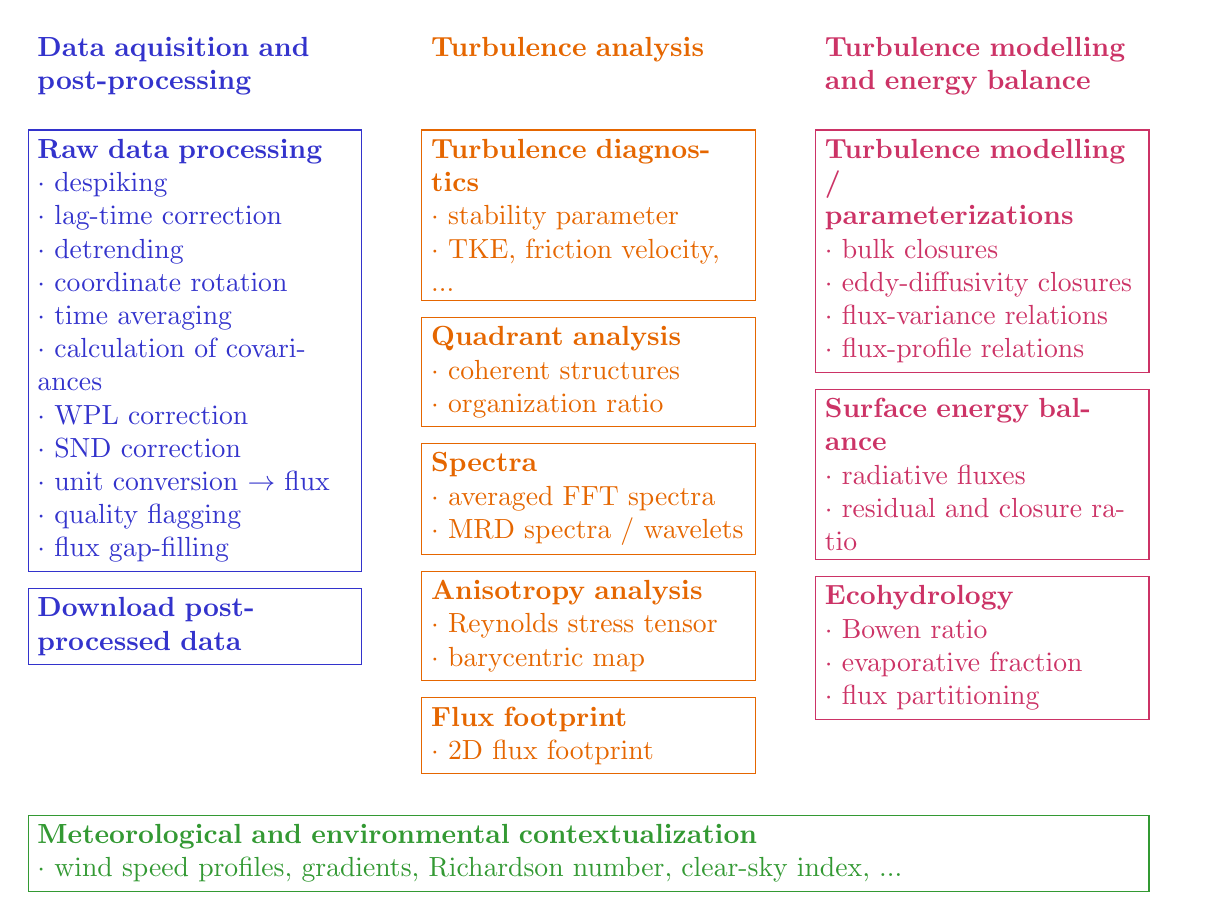
\begin{tikzpicture}
				\node(data) [text width = 4cm,madrid,anchor=north west] at (0,0) { \textbf{Data aquisition and post-processing}} ;
				\node(analysis) [text width = 4cm, orange,anchor=north west] at (5,0) { \textbf{Turbulence analysis} };
				\node(application) [text width = 4.5cm,darkred,anchor=north west] at (10,0) { \textbf{Turbulence modelling and energy balance} };
				
				
				%--------------------------------------------------------------------
				\node(raw) [text width = 4cm,madrid,draw,anchor=north west] at (0,-1.3) { \textbf{Raw data processing} \\
				$\cdot$ despiking \\
				$\cdot$ lag-time correction \\
				$\cdot$ detrending \\
				$\cdot$ coordinate rotation \\
				$\cdot$ time averaging \\
				$\cdot$ calculation of covariances \\
				$\cdot$ WPL correction \\
				$\cdot$ SND correction \\
				$\cdot$ unit conversion $\rightarrow$ flux \\
				$\cdot$ quality flagging \\
				$\cdot$ flux gap-filling 
				} ;
				
				\node(download) [below=0.2cm of raw, text width = 4cm,madrid,draw]  { \textbf{Download post-processed data} 
				} ;
				
				
				%---------------------------------------------------------------------
				\node(diagnostics) [text width = 4cm,orange,draw,anchor=north west]  at (5,-1.3) { \textbf{Turbulence diagnostics} \\
				$\cdot$ stability parameter \\
				$\cdot$ TKE, friction velocity, ...  
				} ;
			   \node(qa) [text width = 4cm,orange,draw,below=0.2cm of diagnostics] { \textbf{Quadrant analysis} \\
			   	$\cdot$ coherent structures \\
			   	$\cdot$ organization ratio 
			   } ;
				\node(spectra) [text width = 4cm,orange,draw,below=0.2cm of qa] { \textbf{Spectra} \\
					$\cdot$ averaged FFT spectra\\
					$\cdot$ MRD spectra / wavelets
				} ;
				\node(aniso) [text width = 4cm,orange,draw,below=0.2cm of spectra] { \textbf{Anisotropy analysis} \\
					$\cdot$ Reynolds stress tensor\\
					%$\cdot$ turbulence anisotropy \\
					$\cdot$ barycentric map
				} ;
				\node(footprint) [text width = 4cm,orange,draw,below=0.2cm of aniso] { \textbf{Flux footprint} \\
					$\cdot$ 2D flux footprint
				} ;
			
				%---------------------------------------------------------------
				
				\node(param) [text width = 4cm,darkred,draw,anchor=north west]  at (10,-1.3) { \textbf{Turbulence modelling / \\ parameterizations} \\
					$\cdot$ bulk closures  \\
					$\cdot$ eddy-diffusivity closures \\
					$\cdot$ flux-variance relations \\  
					$\cdot$ flux-profile relations
				} ;
				\node(seb) [text width = 4cm,darkred,draw,below=0.2cm of param] { \textbf{Surface energy balance} \\
					$\cdot$ radiative fluxes \\
					$\cdot$ residual and closure ratio
				} ;
				\node(hyrdo) [text width = 4cm,darkred,draw,below=0.2cm of seb] { \textbf{Ecohydrology} \\
					$\cdot$ Bowen ratio \\
					$\cdot$ evaporative fraction\\
					$\cdot$ flux partitioning
				} ;
			
			
				%----------------------------------------------------------
			 	\node(meteo) [text width = 14cm,darkgreen,anchor=north west,draw] at (0,-10) { \textbf{Meteorological and environmental contextualization} \\
			 	$\cdot$ wind speed profiles, gradients, Richardson number, clear-sky index, ...} ;

			
				%\draw[->, >=stealth',line width=1.5pt,text width=5cm, align=left] (start) -- (rans) node[midway,right] {\textbf{apply}: \\Reynolds average \\ Boussinesq approximation\\hydrostatic approximation} ;	
				
			\end{tikzpicture}
			\centering

		\end{figure}

\end{document}